\section{Einleitung}


\subsection{Arten von Strahlung}

In diesem Versuch werden $\beta-$und $\gamma-$Zerfälle gemessen.
Diese sind zwei von drei Arten den radioaktiven Zerfalls, die Dritte
Art ist die $\alpha-$Strahlung. Bei der $\alpha-$Strahlung handelt
es sich um Heliumatomkerne, bestehend aus zwei Protonen und zwei Neutronen,
die aus dem radioaktiven Atom hinausgeschleudert werden, dabei nimmt
die Masse des Atoms um vier atomare Masseneinheiten ab (4 atomare
Masseneinheiten=4u$\approx6,64\cdot10^{-27}kg$) und die Ordnungszahl
wird um zwei verringert, dadurch entsteht ein neues Element. Die $\alpha$-
Strahlung besitzt diskrete Energiebeträge.

Da die $\alpha-$Strahlung nicht in diesem Versuch vorkommt, wird
nicht weiter darauf eingegangen.

Bei der $\beta-$Strahlung gibt es zwei mögliche Zerfälle die stattfinden
können. Zum einen der $\beta^{-}$-Zerfall bei dem ein Neutron im
Atomkern zu einem Proton sowie Elektron und einem Neutrino zerfällt,
dabei verbleibt das Proton im Atomkern, das Elektron ist das Teilchen,
welches als $\beta$-Strahlung gemessen werden kann, das Neutrino
ist nur sehr schwer nachweisbar. Neben dem $\beta^{-}$-Zerfall gibt
es noch den $\beta^{+}$-Zerfall bei dem ein Proton in ein Neutron,
ein Positron und ein Neutrino zerfällt, das Positron kann als $\beta$-Strahlung
gemessen werden, auch hier ist das Neutrino nur sehr schwer nachweisbar.

Im Gegensatz zur $\alpha$- und $\gamma$- Strahlung besitzt die $\beta$-
Strahlung keine diskreten sondern kontinuierliche Energiebeträge bis
hin zu einer gewissen Maximalenergie, dieses Phänomen liegt an dem
Neutrino, welches die fehlende Energie aufnimmt.

Die $\gamma$- Strahlung besteht aus hochenergetischen Photonen, den
sogenannten $\gamma$- Quanten, diese entstehen aus angeregten Atomen
dadurch, dass die Protonen und Neutronen im Atomkern ihren Energiezustand
ändern und die Energiedifferenz wird als $\gamma$- Quant ausgesendet,
diese haben wie die $\alpha$- Strahlung diskrete Energiebeträge.


\subsection{Absorption von Strahlung}


\subsubsection{Absorption von $\gamma$- Strahlung}

Bei der Absorption von $\gamma$- Strahlung gibt es drei Absorptionsmechanismen,
dem Photoeffekt bei welchem das $\gamma$-Quant von einem Atom absorbiert
wird und dieses emittiert ein Elektron auf einer der inneren Schalen
der Elektronenhülle. Der zweite Absorptionsmechanismus ist der Comptoneffekt,
bei dem eine inelastische Streuung des $\gamma$- Quants stattfindet,
in welchem es die Frequenz und die Richtung ändert. Der dritte Absorptionsmechanismus
ist die Paarbildung, dort entstehen aus einem $\gamma$- Quant hoher
Energie ( E>2$m_{e}c^{2}\approx 1MeV$) ein Elektron und ein Positron.

Der Absorptionskoeffizient $\mu$setzt sich aus allen drei Absorptionsmechanismen
zusammen
\begin{equation}
	\mu=\mu_{Photo}+\mu_{Compton}+\mu_{Paar}
\end{equation}


diese Größe ist ebenfalls vom Absorbermaterial abhängig.

Treffen nun N $\gamma$- Quanten auf einen Absorber der Dicke \emph{dx
}so wird folgende Relation erhalten
\begin{equation}
	dN=-\mu Ndx
\end{equation}


gelegentlich wird auch die Massenbelegung $\rho$eingeführt, welches
die Dichte des Absorbermaterials darstellt. Dadurch wird $\mu$zu
$\mu_{m}=\frac{\mu}{\rho}$, also 
\begin{equation}
	dN=-\mu_{m}N\rho dx
\end{equation}


durch Integration ergibt sich eine exponentielle Abnahme der Teilchenzahl
mit der Absorberdicke.

\begin{equation}
	N(x)=N_{0}\cdot exp(-\mu)=N_{0}\cdot exp(-\mu_{m}\rho x)
\end{equation}



\subsubsection{Absorption von $\beta-$Strahlung}

Die exponentielle Abnahme gilt nicht für $\beta-$Strahlung, der Grund
hierfür ist, dass die $\beta-$Absorption nicht durch einen einzigen
Prozess erfolgt. Die Elektronen verlieren ihre Energie durch mehrere
inelastische Stöße mit den Atomen des Absorbermaterials, auch ist
es möglich, dass sie durch eine Richtungsänderung aus dem Strahl ausscheiden.
Somit wird für $\beta-$Strahlung die ,,mittlere Reichweite`` $R_{m}$
definiert, dass ist die Absoberdicke bei der noch 50\% der Anfangsstrahlung
vorhanden ist, daneben wird die ,,praktische Reichweite`` definiert,
diese ist als Schnittpunkt des extrapolierten linearen Abfalls der
Reichweitenverteilung mit der Achse \emph{N(x)=0 }definiert.


\subsection{Nachweis der Strahlung}

Zum Nachweis der Strahlung wird ein Geiger-Müller-Zählrohr verwendet.
Im luftdichten Zählrohr befindet sich Argon unter einem Druck von
ungefähr 100mbar und Alkoholdampf, welches einen Partialdruck von
etwa 10mbar hat. Es wird praktisch jedes $\alpha$- und $\beta$-Teilchen
vom Zählrohr erfasst, die $\gamma$- Strahlen werden mit einer kleineren
Menge nachgewiesen.

Im wesentlichen wird der Nachweismechanismus durch eine Ionisierung
eines Argon Atoms, da sich im Inneren des Zählrohrs ein elektrisches
Feld befindet, wird das Ionenpaar, welches aus Elektron und dem Argon-Ion
besteht, jeweils zur Anode bzw. zur Kathode hin beschleunigt. 

Auf diesem Weg ionisieren das Elektron andere Atome und es kommt zu
einer Entladungslawine. Wenn das Argon-Ion auf die Zählrohrwand auftrifft,
werden Sekundärelektronen emittiert, diese tragen zur Erhaltung des
Entladungsprozesses bei. Die Alkoholmoleküle stoppen diesen Entladungsprozess.

Nach jedem Entladungsstoß bleibt das Zählrohr für einige $10^{-4}s$
für neue Teilchen unempfindlich, diese Zeit wird ,,Totzeit`` genannt.
Erst nach diese Zeit kann ein neues Teilchen detektiert werden.


\subsection{Poisson-Verteilung}

Der Erfahrung nach ist die Rate mit der Radioaktive-Zerfälle stattfinden
mit der Poisson-Verteilung beschreibbar. Die Poisson-Verteilung geht
aus der Binomial-Verteilung für eine große Zahl von Objekten und einer
geringen Ereigniswahrscheinlichkeit hervor. Die allgemeine Gleichung
lautet 
\begin{equation}
	\psi_{n}=\frac{\bar{k}^{k}\cdot e^{-\bar{k}}}{k!}\label{eq:Poisson-Verteilung allgemein}
\end{equation}


$\bar{k}$ entspricht dem Erwartungswert 
\begin{equation}
	\bar{k}=np
\end{equation}


$n$ entspricht hier der Anzahl der Atome und $p$ entspricht der
Wahrscheinlichkeit für einen Zerfall.

Bei einer Poisson-Verteilung sind Erwartungswert und Varianz gleich.

\begin{equation}
	\sigma^{2}=np=\bar{k}
\end{equation}


Um nun die Poisson-Verteilung auf den radioaktiven Zerfall anzuwenden
muss der Mittelwert für die gemessenen Zerfälle $\bar{N}$ bestimmt
werden. Dazu werden n-mal die Zahl der zerfallenen Kerne $N_{i}$
jeweils in einem festen Zeitintervall $\triangle T$ gemessen. Dann
wird aus \ref{eq:Poisson-Verteilung allgemein} 
\begin{equation}
	\psi(N)=\frac{\bar{N}^{N}\cdot e^{-\bar{N}}}{N!} \label{eq:pois_id}
\end{equation}


darauf ergibt sich für die mittlere Streuung,
\begin{equation}
\sigma=\sqrt{\bar{N}} \label{eq:std_abw}
\end{equation}


dieses wird $\sqrt{N}-Gesetz$ genannt.

Um  bei den Versuchen einen statistischen Fehler von maximal $ \SI{3}{\percent} $ zu erreichen, darf die Varianz nicht mehr als $ \SI{3}{\percent} $ der Messgröße betragen ($ 1\sigma $ Umgebung $ \sim \SI{68.3}{\percent} $ Sicherheit)
\begin{align}
	&\frac{\sigma}{N} = \frac{\sqrt{N}}{N} = \frac{1}{\sqrt{N}} \stackrel{!}{\leq} \SI{3}{\percent} \notag \\
	\Rightarrow & N \geq \frac{1}{(\SI{3}{\percent})^2} \approx 1112 \label{eq_n_pulszahl}
\end{align}


\newpage
\section{Versuchsteil}
Der Versuchsaufbau ist bei jedem der folgenden Versuche der gleiche. Ausgetauscht werden lediglich die Absorber und die Strahlenquelle. Als Strahlenquelle wird entweder ein \isotope[90]{Sr} $ \beta $-Strahler oder ein \isotope[137]{Cs} $ \gamma $-Strahler verwendet. Auf einen Geiger-Müller-Zähler mit angeschlossenem Zählwerk und Stoppuhr werden die jeweilige Strahlenquelle in vernachlässigbar geringen Abstand ausgerichtet und dazwischen gegebenen Falls die zu prüfenden Absorber platziert. Die gerade nicht verwendeten Strahlenquellen werden gegen die Wand ausgerichtet, um die Messung nach Möglichkeit nicht zu verfälschen.

\subsection{Messung der Zählrohrcharakteristik}
In diesem Versuch ist das Ziel, die Zählrohrcharakteristik zu bestimmen. Das heißt, die Abhängigkeit der gemessenen Strahlenpulse von der am Geiger-Müller-Zähler angelegten zu bestimmen. Dazu wird der zuvor beschriebene Aufbau mit dem $ \beta $-Strahler verwendet und zunächst die höchste Spannung gesucht, bei der keine Strahlung gemessen wird. Daraufhin wird ab etwa $ \SI{50}{\volt} $ über dieser Spannung die Impulsrate gemessen. Um eine statistische Unsicherheit von maximal $ \SI{3}{\percent} $ zu erreichen werden nach \eqref{eq_n_pulszahl} mindestens $ 1112 $ Strahlenpulse gemessen. Beim einstellen der Spannung muss gegebenen Falls beachtet werden, dass die es nicht zur selbständigen Gasentladung kommt und das Zählrohr somit geschädigt wird. Jedoch war es mit unserem Versuchsaufbau nicht möglich, solche Spannungen zu erreichen. \\
Unsere Messwerte sind Tabelle \ref{tab:mess_1} zu entnehmen

\begin{table}[h!]
\begin{tabular}{c|c|c|c|c}
Spannung $ [\si{\volt}] \pm \num{12.5} $ & Impulsrate & Zeit $ [\si{\second}] \pm 1$ & Impulszahl $ [\si{\per\second}] $ & Unsicherheit $ [\si{\per\second}] $ \\ \hline
$ 350 $ & $ 1112 $ & $ 101 $ & $ \num{11.0099} $ & $ \num{0.3477} $ \\
$ 400 $ & $ 1116 $ & $ 103 $ & $ \num{10.8350} $ & $ \num{0.3410} $ \\
$ 450 $ & $ 1117 $ & $ 98 $ & $ \num{11.3980} $ & $ \num{0.3604} $ \\
$ 500 $ & $ 1115 $ & $ 104 $ & $ \num{10.7212} $ & $ \num{0.3373} $ \\
\end{tabular}
\caption{Messwerte Zählrohrcharakteristik}
\label{tab:mess_1}
\end{table}

Nach unserer Messung ist die Änderung der Impulsrate im Bereich $ \SI{350}{\volt} $ bis $ \SI{500}{\volt} $ für uns unmessbar klein. Die Abweichung der Messwerte bewegt sich lediglich im Unsicherheitsbereich obwohl diesem nur eine $ 1\sigma $-Umgebung zu Grunde liegt. Somit könnten alle folgenden Versuche mit einer beliebigen Spannung zwischen $ \SI{350}{\volt} $
 und $ \SI{500}{\volt} $ durchgeführt werden. Dennoch haben wir uns darauf festgelegt, eine Spannung von $ \SI{500}{\volt} $ in allen folgenden Teilen beizubehalten.
\subsection{Messung der Untergrundpulse}
\subsubsection{Häufigkeitsverteilung der Untergrundpulse}
Bei diesem Versuchsteil werden die Untergrundpulse gemessen, die durch natürliche Strahlenquellen auftreten. Der Anfangs beschriebene Versuchsaufbau wird dazu ohne Strahlenquelle und Absorber betrieben. \\
Im ersten Teil dieses Versuches wird $ 100 $ mal die Strahlung in $ \SI{10}{\second} $ gemessen. Wir erhielten die Wahrscheinlichkeitsverteilung gemäß Abbildung \ref{fig:haeuf_hint_1}.

\begin{figure}[h!]
	\centering
	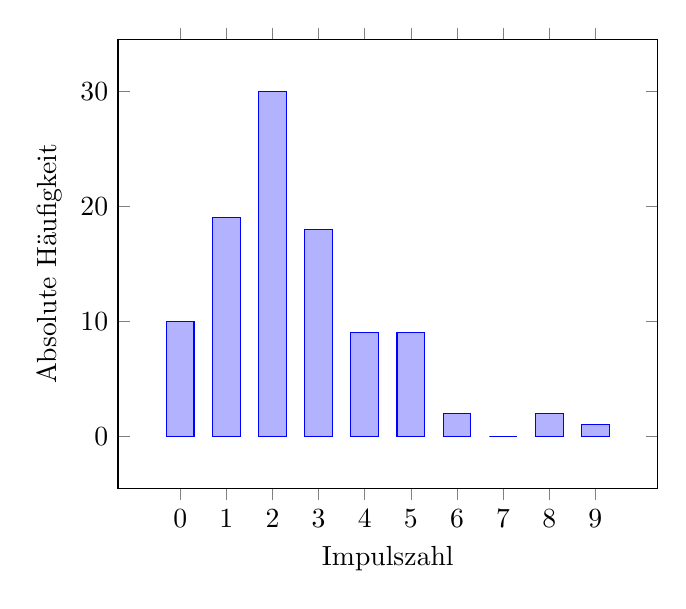
\begin{tikzpicture}
\begin{axis} [
enlargelimits=.15,
ybar,
%symbolic x coords={excellent, good, neutral},
xtick = data,	
xlabel={Impulszahl},
ylabel={Absolute Häufigkeit}
]
\addplot coordinates {(0, 10)
	(1, 19)
	(2, 30)
	(3, 18)
	(4, 9)
	(5, 9)
	(6, 2)
	(7, 0)
	(8, 2)
	(9, 1)
};
\end{axis}
\end{tikzpicture}
	\caption{Häufigkeitsverteilung der Impulszahlen}
	\label{fig:haeuf_hint_1}
\end{figure}

Die mittlere Impulszahl $ \bar N $ ist die Gesamtzahl der Impulse geteilt durch die Anzahl der Messungen. Diese beträgt bei uns $ \bar N = \num{2.51} $. Da von einer Poisson-Verteilung ausgegangen werden kann beträgt die Standard-Abweichung nach \eqref{eq:std_abw} $ \sigma = \sqrt{\bar N} \approx \num{1.585} $.\\
Aus \eqref{eq:pois_id} lässt sich damit die erwartete Wahrscheinlichkeitsverteilung bestimmen. In Abbildung \ref{fig:a2_rech} ist dies gegen die im Experiment ermittelten Häufigkeiten aufgetragen.

\begin{figure}[h!]
\centering
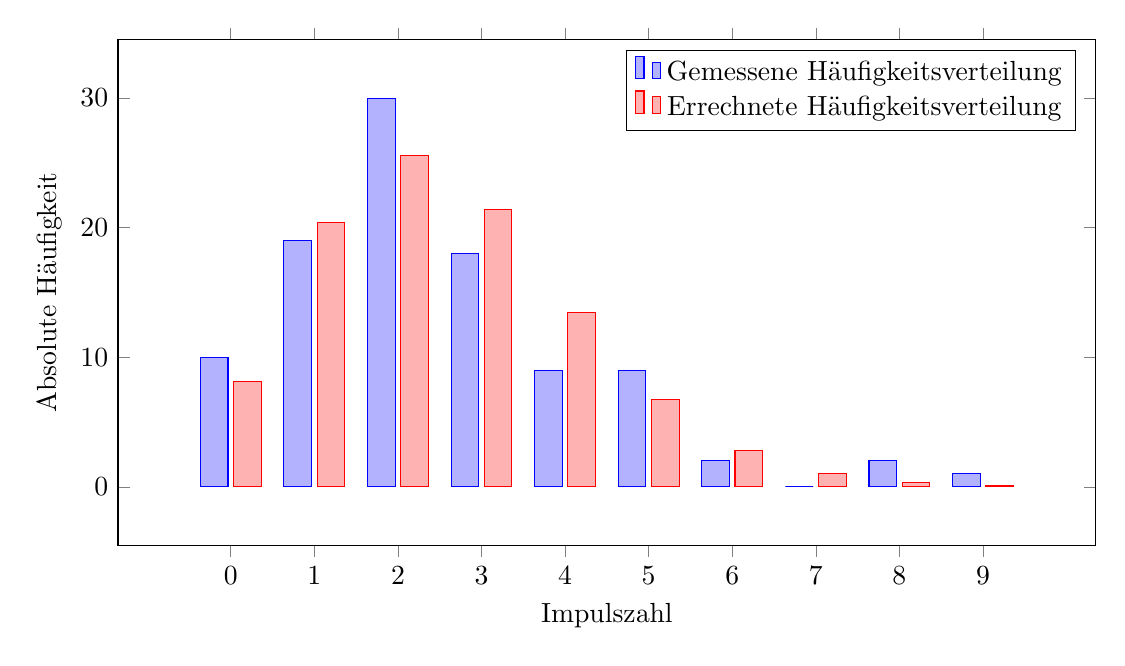
\begin{tikzpicture}[]
\begin{axis} [
width=14cm,
height = 8cm,
enlargelimits=.15,
ybar,
%bar width = 5pt,
%symbolic x coords={excellent, good, neutral},
%nodes near coords,
xtick = data,
xlabel={Impulszahl},
ylabel={Absolute Häufigkeit},
]
\addplot coordinates {(0, 10)
	(1, 19)
	(2, 30)
	(3, 18)
	(4, 9)
	(5, 9)
	(6, 2)
	(7, 0)
	(8, 2)
	(9, 1)
};
\addlegendentry{Gemessene Häufigkeitsverteilung};
\addplot table[x = x, y=y] {
x y
0	8.1268239241
1	20.3983280495
2	25.5999017021
3	21.4185844241
4	13.4401617261
5	6.7469611865
6	2.822478763
7	1.0120602422
8	0.317533901
9	0.0885566768
};
\addlegendentry{Errechnete Häufigkeitsverteilung};
\end{axis}
\end{tikzpicture}
\caption{Rechnerische und gemessene Wahrscheinlichkeitsverteilung der Impulszahlen}
\label{fig:a2_rech}
\end{figure}

Die Poisson-Verteilung gibt im Wesentlichen die Messwerte richtig wieder. Gerade bei Wahrscheinlichkeits-Experimenten kann man nicht erwarten, dass das mathematisch wahrscheinlichste Ergebnis auch eintritt auf Grund von statistischen Fehlern. Zudem ist $ N = 100 $ auch gerade für die Poisson-Verteilung noch eine relativ kleine Stichprobe. Dies zeigt sich auch durch die relativ große Standardabweichung: selbst im mathematischen Modell ist bereits eine verhältnismäßig große Abweichung eingerechnet. In Anbetracht dieser Punkte kann die Poisson-Verteilung als gutes Modell angesehen werden.

\subsubsection{Korrekturfaktor für Untergrundpulse}
Aus den Untergrundpulsen entsteht für alle anderen Experimente ein Störfaktor, da der Geiger-Müller-Zähler nicht zwischen der Strahlung des Präperats und der Untergrundstrahlung unterscheidet. Um diesen Fehler zu bereinigen wird in diesem Versuchsteil die Untergrundstrahlungsrate ermittelt. Dazu wird die Zeit gemessen, die gebraucht wird um ohne Präperat mehr als $ 500 $ Pulse zu messen.\\
In $ \SI{2070(1)}{\second} $ haben wir $ 501 $ Pulse gemessen. Daraus ergibt sich eine Pulsrate von $ \SI{.2420(108)}{\per\second} $. Diese muss von allen folgenden gemessenen Pulsraten abgezogen werden.

\subsection{Absorbtion von $ \beta $-Strahlung}

Zur Untersuchung von $ \beta $-Strahlung wird in den anfangs beschriebenen Versuchsaufbau ein \isotope[90]{Sr} eingesetzt, das $ \beta $-Strahlung von maximal $ E_max = \SI{.54}{\MeV} $ ausstrahlt. Dann werden Aluminium-Absorber mit verschiedenen dicken eingesetzt, um das Absorbtionsverhalten zu ermitteln. Um den statistischen Fehler unter $ \SI{3}{\percent} $ zu halten werden auch hier mindesten $ 1112 $ Pulse gezählt. Wir erhielten die folgenden Ergebnisse. Die einzelnen Messwerte sind im Laborbuch zu finden

\begin{table}[h!]
\centering
\begin{tabular}{c|c|c}
Schichtdicke $ [\si{\micro\meter}] $ & Impulsrate $ [\si{\per\second}] $ & Unsicherheit $ [\si{\per\second}] $ \\\hline
$ 0 $ & $ \num{10.4791} $ & $ \num{0.3480} $ \\ 
$ 50 $ & $ \num{9.8030} $ & $ \num{0.3249} $ \\
$ 107 $ & $ \num{9.7847} $ & $ \num{0.3231} $ \\
$ 165 $ & $ \num{8.1339} $ & $ \num{0.2695} $ \\
$ 215 $ & $ \num{6.8471} $ & $ \num{0.2280} $ \\
$ 330 $ & $ \num{6.2119} $ & $ \num{0.2069} $ \\
$ 520 $ & $ \num{5.0722} $ & $ \num{0.1718} $ \\
$ 770 $ & $ \num{3.6943} $ & $ \num{0.1295} $
\end{tabular}
\caption{Messwerte Absorbtion von $ \beta $-Strahlung an Aluminium}
\label{tab:abs_alu}
\end{table}

Ohne einen Absorber beträgt die Impulsrate für den $\beta$- Strahler
bei 500V$\pm$12,5V ungefähr 11 Zerfälle pro Sekunde. Nun werden mit
zunehmender Schicktdicke Aluminiumabsober vor das Präperat gestellt..
Die Messdaten lassen sich in den folgenden Diagrammen Abbildungen \ref{fig:alu_lin} und \ref{fig:alu_log} aufzeigen,

\begin{figure}[h!]
\centering
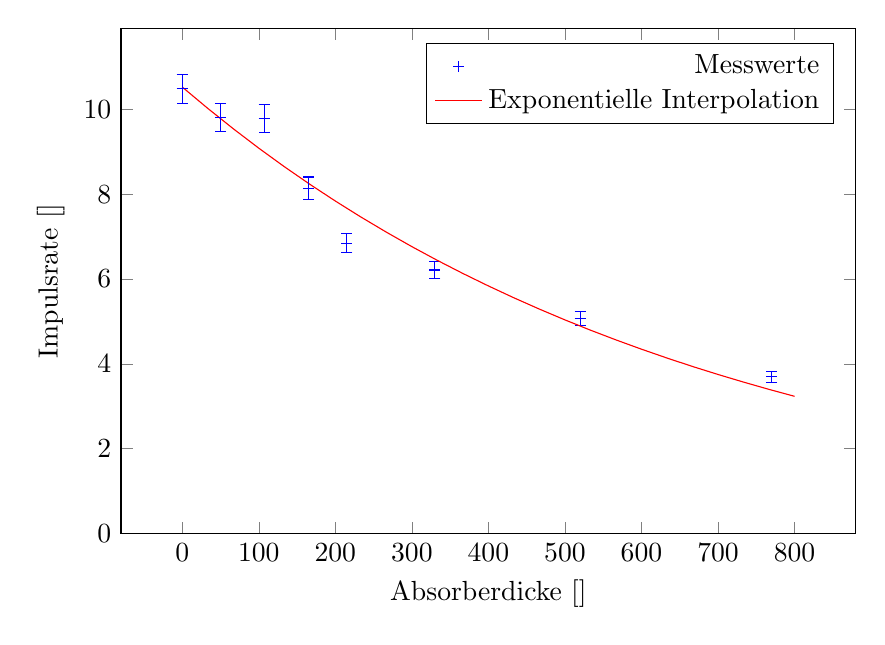
\begin{tikzpicture}
\begin{axis} [
%enlargelimits=.15,
%ybar,
%symbolic x coords={excellent, good, neutral},
%xtick = data,
width=.9\textwidth,
height = 8cm,
error bars/y dir = both,
error bars/y explicit,
%only marks,
ymin = 0,
%ymode=log,
xlabel={Absorberdicke [\si{\micro\meter}]},
ylabel={Impulsrate [\si{\per\second}]},
legend style = {legend pos =  north east, cells={anchor=east}}
]
\addplot+ [mark = +, only marks] table[x = x, y= y, y error = yerror]  {
x	y	yerror
0	10.4791248606	0.3480304704
50	9.8030160595	0.3249560292
107	9.7847567288	0.3231269543
165	8.1339108641	0.2695473226
215	6.847142989	0.228052825
330	6.211994003	0.206946066
520	5.0722567288	0.171892932
770	3.6943667742	0.1295697446
};
\addlegendentry{Messwerte};
\addplot+[no marks, domain=0:800] {10.52378637*exp(-1474.24606886e-6*x)};
\addlegendentry{Exponentielle Interpolation};
\end{axis}
\end{tikzpicture}
\caption{Absorberdicke-Pulsrate-Diagramm für Aluminium mit linearer Skala}
\label{fig:alu_lin}
\end{figure}

\begin{figure}[h!]
\centering
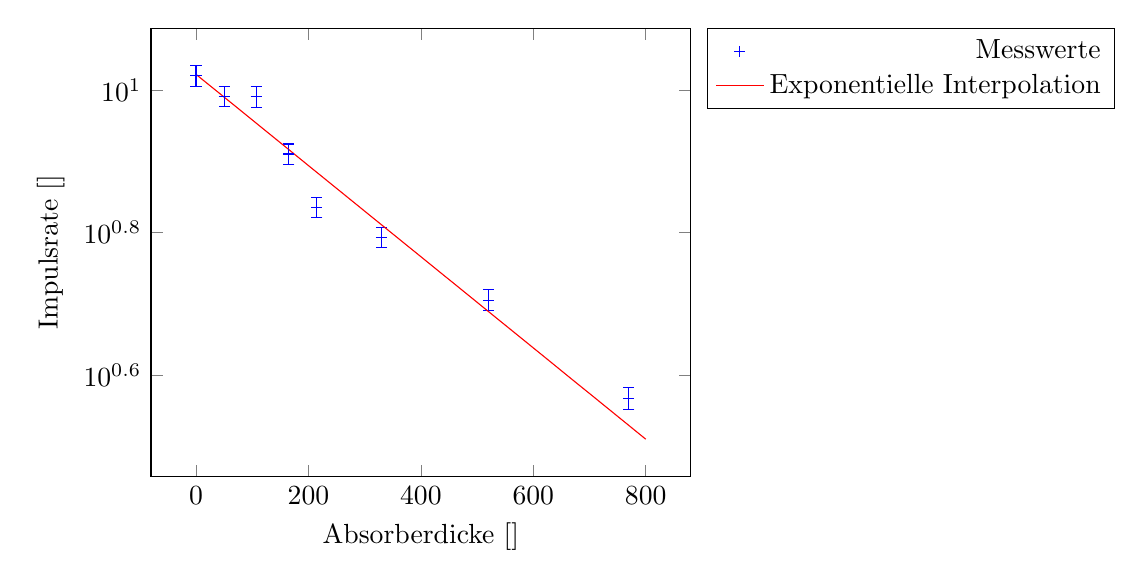
\begin{tikzpicture}
\begin{axis} [
%enlargelimits=.15,
%ybar,
%symbolic x coords={excellent, good, neutral},
%xtick = data,
error bars/y dir = both,
error bars/y explicit,
%only marks,
%ymin = 0,
ymode=log,
xlabel={Absorberdicke [\si{\micro\meter}]},
ylabel={Impulsrate [\si{\per\second}]},
legend style = {legend pos = outer north east, cells={anchor=east}}
]
\addplot+ [mark = +, only marks] table[x = x, y= y, y error = yerror]  {
x	y	yerror
0	10.4791248606	0.3480304704
50	9.8030160595	0.3249560292
107	9.7847567288	0.3231269543
165	8.1339108641	0.2695473226
215	6.847142989	0.228052825
330	6.211994003	0.206946066
520	5.0722567288	0.171892932
770	3.6943667742	0.1295697446
};
\addlegendentry{Messwerte};
\addplot+[no marks, domain=0:800] {10.52378637*exp(-1474.24606886e-6*x)};
\addlegendentry{Exponentielle Interpolation};
\end{axis}
\end{tikzpicture}
\caption{Absorberdicke-Pulsrate-Diagramm für Aluminium mit log Skala}
\label{fig:alu_log}
\end{figure}

in Realität nähern sich die Werte der Achse für die Impulsrate nur
asymptotisch an den Nullpunkt an.

Wird nun extrapoliert, d.h. das Verhalten der Impulsrate wird über
den gesicherten Bereich hinaus (approximiert) bestimmt, kann die praktische
Reichweite bestimmt werden. 

Dafür wird angenommen, dass die Impulsrate um 1,5$\frac{Zerf\ddot{a}lle}{Sekunde}$
sinkt, wenn die Dicke des Aluminumabsorbers um 250$\mu m$ zunimmt. 

Bei dem letzten gemessenen Wert beträgt die Impulsrate in sehr guter
Näherung 4$\frac{Zerf\ddot{a}lle}{Sekunde}$ bei einer Absorberdicke
von 770$\mu m$. Um nun die Dicke des Absorbers für 0$\frac{Zerf\ddot{a}lle}{Sekunde}$
abzuschätzen werden die Annahmen verwendet, also müssten zusätzliche
650$\mu m$ Aluminumabsorber hinzugefügt werden.

Somit beträgt die praktische Reichweite der $\beta-$Strahlung bei
Aluminum 1420$\mu m$.

\subsubsection{Absorbtion an Gummi und Plexiglas}
Für Gummi und Plexiglas waren nur wenige Messwerte möglich, da nur zwei Absorber für Gummi und nur einer für Plexiglas zur Verfügung standen. Diese Messwerte werden analog zu den vorherigen erfasst, indem der jeweilige Absorber eingesetzt und mindesten $ 1112 $ Pulse gemessen werden.
Die Ergebnisse stehen in Tabelle \ref{tab:abs_gum}. Die einzelnen Messwerte sind im Laborbuch zu finden.
\begin{table}[h!]
\centering
\begin{tabular}{c|c|c|c}
& Schichtdicke $ [\si{\centi\meter}] $ & Impulsrate $ [\si{\per\second}] $ & Unsicherheit $ [\si{\per\second}] $ \\\hline
& $ 0 $ & $ \num{10.4791} $ & $ \num{0.3480} $ \\ 
Plexiglas &  $ \num{.5} $ & $ \num{0.9588} $ & $ \num{0.0469} $ \\
Gummi & $ \num{.15} $ & $ \num{3.7130} $ & $ \num{0.1286} $ \\
	  &	$ \num{.30} $ & $ \num{1.0282} $ & $ \num{0.0489} $
\end{tabular}
\caption{Messwerte Absorbtion von $ \beta $-Strahlung an Gummi und Plexiglas}
\label{tab:abs_gum}
\end{table}
Legt man eine Funktion der Form $ N(d) = N_0 \mathrm{e}^{-\mu d} $ durch die Messwerte, so erhält man für Plexiglas $ \mu \approx \SI{4.7828}{\per\centi\meter} $ und für Gummi $ \mu \approx \SI{7.1720}{\per\centi\meter} $. Wegen $ \mathrm{e}^{-\mathrm{ln} 2} = \frac{1}{2} $ ist die Halbwertsdicke gegeben durch $ R_m = \frac{\mathrm{ln}2}{\mu} $. Somit ist die Halbwertsdicke für Plexiglas $ R_m \approx \SI{0.1450}{\centi\meter} $ und für Gummi $ R_m \approx \SI{.0966}{\centi\meter} $.\\
Die Halbwertsdicke dieser beiden Materialien ist erwartungsgemäß um Größenordnungen über der von Aluminium. Aluminium als Metall reagiert und stärker auf Ladungsträger wie die Elektronen der $ \beta $-Strahlung und stellt daher für diese ein größeres Hindernis da.

\subsection{Absorbtion von $ \gamma $-Strahlung}
Im letzten Versuchsteil wurde das $\gamma$-Präperat vor das Zählrohr
gestellt um, deren Zerfälle zu bestimmen. Als Absorber wurden bis zu vier Bleiplatten mit einer Dicke von jeweils $ \SI{5.0(1)}{\milli\meter} $ verwendet. Die Ergebnisse stehen in Tabelle \ref{tab:abs_pb}. Die einzelnen Messwerte sind im Laborbuch zu finden.
\begin{table}[h!]
\centering
\begin{tabular}{c|c|c}
Schichtdicke $ [\si{\milli\meter}] $ & Impulsrate $ [\si{\per\second}] $ & Unsicherheit $ [\si{\per\second}] $ \\\hline
$ 0 $ & $ \num{8.9811} $ & $ \num{0.2972} $ \\
$ \num{5.0(1)} $ & $ \num{5.0032} $ & $ \num{0.1700} $ \\
$ \num{10.0(2)} $ & $ \num{3.0248} $ & $ \num{0.1091} $ \\
$ \num{15.0(3)} $ & $ \num{1.8822} $ & $ \num{0.0727} $ \\
$ \num{20.0(4)} $ & $ \num{1.0670} $ & $ \num{0.0500} $
\end{tabular}
\caption{Messwerte Absorbtion von $ \gamma $-Strahlung an Blei}
\label{tab:abs_pb}
\end{table}

Anhand von Abbildung \ref{fig:pb_log} ist durch die logarithmische Darstellung der
Impulsrate eine lineare Abnahme der Impulse mit der Absorberdicke
sichtbar. Würde die Impulsrate auf einer linearen Achse dargestellt
werden, so wäre eine exponentielle Abnahme zu sehen.

\begin{figure}[h!]
\centering
\begin{tikzpicture}
\begin{axis} [
%enlargelimits=.15,
%ybar,
%symbolic x coords={excellent, good, neutral},
%xtick = data,
error bars/y dir = both,
error bars/y explicit,
%only marks,
%ymin = 0,
ymode=log,
%mark = +,
%log ticks with fixed point,
xlabel={Absorberdicke $ [\si{\milli\meter}] $},
ylabel={Impulsrate [\si{\per\second}]},
legend style = {legend pos = outer north east, cells={anchor=east}}
]
\addplot+[mark = +, only marks,
	error bars/x dir = both, error bars/x fixed relative=.02,] table[x = x, y= y, y error = yerror]  {
x	y	yerror
0	8.9811115104	0.2972302496
5	5.0032540334	0.1700432809
10	3.0248331846	0.1091601283
15	1.8822953388	0.0727996721
20	1.0670191931	0.0500643354
};
\addlegendentry{Messwerte}
\addplot+[no marks, domain=0:20,] 
	{8.9107847*exp(-0.10837785*x)};
\addlegendentry{Exponentielle Interpolation};
\end{axis}
\end{tikzpicture}
\caption{Absorberdicke-Pulsrate-Diagramm für Blei mit log Skala}
\label{fig:pb_log}
\end{figure}

Um daraus den Absorptionskoeffizienten $\mu$zu bestimmen, kann die
Formel für die $\gamma-$Absorption einfach nach $\mu$aufgelöst werden.
Es folgt:

\[
\mu=\frac{ln\left(\frac{N_{0}}{N(x)}\right)}{x}=-0,10837785\frac{1}{mm}
\]


für den Massenabsorptionskoeffizienten $\mu_{m}$folgt daraus,
\[
\mu_{m}=\frac{\mu}{\rho_{Blei}}=\frac{-0,10837785\frac{1}{mm}}{0,011342g/mm^{3}}\approx-9,55\frac{mm^{2}}{g}
\]


diese Werte gelten für $\gamma$-Quanten die eine Energie von $ \SI{.66}{\MeV} $
haben.
